\section{Question 2}
Train and evaluate a Decision Tree (DT) on the same classification problem chosen in Question 1. 
Present the resulting tree (depth, rule-based description) 
and compare its performance with the results obtained in Question 1.

\noindent\rule{\textwidth}{.5pt}

\noindent\textbf{Dataset description.}
    The dataset chosen is Michael J. Fox Foundation's Parkinson's Progression Markers Initiative (PPMI)
    bank of raw sequencing reads from blood samples.
    %
    Over 4000 participants have had their RNA transcripted across several visits,
    and the result of this analysis bundled with other categorical variables 
    (such as age, gender, race, etc.) to form the PPMI dataset.
    %
    As a dataset designed for the study of Parkinson Disease (PD) prediction and identification,
    each patient falls under one of three classes:
    %
    \begin{multicols}{3}
        \begin{itemize}
            \item ``0''/``Case'' if with PD
            \item ``1''/``Control'' if healthy
            \item ``2''/``Other'' if prodromal
        \end{itemize}        
    \end{multicols}

    Of the original 56 columns in the CSV of PPMI patient metadata (\texttt{meta\_data11192021.csv}), 
    4 are diagnostic labels, and 23 were dropped from consideration due to one or more of the following: 
    %
    \begin{enumerate}
        \item [(i)] redundancy (e.g., ``Age (Bin)'', ``Age at diagnosis'');
        \item [(ii)] could not contribute to the cause of PD (e.g., ``Month'' of visit, ``Plate'' of the sample);
        \item [(iii)] are patient identifiers (e.g., ``HudAlphaSampleName'', ``PATNO'');
        \item [(iv)] were sparsely present across samples (e.g., ``UPSIT'').
    \end{enumerate}

    As such, each sample from the dataset consists of 29 features.    
    From this subset of data, features with correlation greater than or equal to 90\% (in absolute value) were dropped.
    
    After the removal of highly-correlated features, the samples are shuffled 
    and finally separated into training, validation, and test sets 
    in splits of 50\%, 25\% and 25\%, respectively.
    
    \Cref{tab:data_ppmi} profiles the sets obtained from the preprocessing of PPMI.
    \Cref{fig:data_preprocessing} shows a flowchart of the preprocessing done to data. 
    \Cref{fig:correlations_ppmi} shows the correlation matrix of the PPMI dataset.
    Since one ``Neutrophils (\%)'' was dropped due to high negative correlation with ``Lymphocytes (\%)'',
    there are 28 features total instead of 29.
    
    \begin{table}[hbp]
        \centering
        \caption{
            PPMI train-validation-test splits. 
            Randomizer seed was fixed at 2421.}
        \label{tab:data_ppmi}
        \begin{tabular}{l rr rr rr}
        \toprule
            \multicolumn{1}{c}{\multirow{2}{*}{Class}}
            & \multicolumn{6}{c}{Absolute and relative amounts within split} \\
        \cmidrule{2-7}
            & \multicolumn{2}{c}{Train} 
            & \multicolumn{2}{c}{Validation} 
            & \multicolumn{2}{c}{Test} \\
        \midrule
            0 (PD) 
                & 183 & 30.30\% 
                & 100 & 33.11\% 
                & 112 & 36.96\% \\
            1 (Healthy)
                & 416 & 68.87\% 
                & 200 & 66.23\% 
                & 189 & 62.38\% \\
            2 (Prodromal)
                & 5 & 0.83\% 
                & 2 & 0.66\% 
                & 2 & 0.66\% \\
        \midrule 
        \multicolumn{1}{c}{Samples}
                & 604 & 49.96\%
                & 302 & 24.98\%
                & 303 & 25.06\% \\
        \bottomrule
        \end{tabular}
    \end{table}
    
    \clearpage
    \begin{figure}[htbp]
        \centering
        \caption{
            Steps taken in this work to prepare data for machine learning algorithms.
        }
        \label{fig:data_preprocessing}
        \begin{tikzpicture}[> = latex]
    \node [startstop] (start) at (0, 0) {Start};
    \node [io, below=1 of start] (1) {Raw data};
    \node [process, right=1 of 1] (2) {Drop non-relevant features};
    \node [process, above=1 of 2] (3) {Drop highly correlated features};
    \node [process, right=1 of 3] (4) {Shuffle sample order};
    \node [io, below=1 of 4] (5) {Train-validation-test split};
    \node [startstop, right=1 of 5] (stop) {Stop};

    \draw [->] (start) -- (1);
    \draw [->] (1) -- (2);
    \draw [->] (2) -- (3);
    \draw [->] (3) -- (4);
    \draw [->] (4) -- (5);
    \draw [->] (5) -- (stop);
\end{tikzpicture}
    \end{figure}
    %
    \begin{figure}[h!]
        \centering
        \caption{Feature correlations found in a subset of PPMI.}
        \label{fig:correlations_ppmi}
        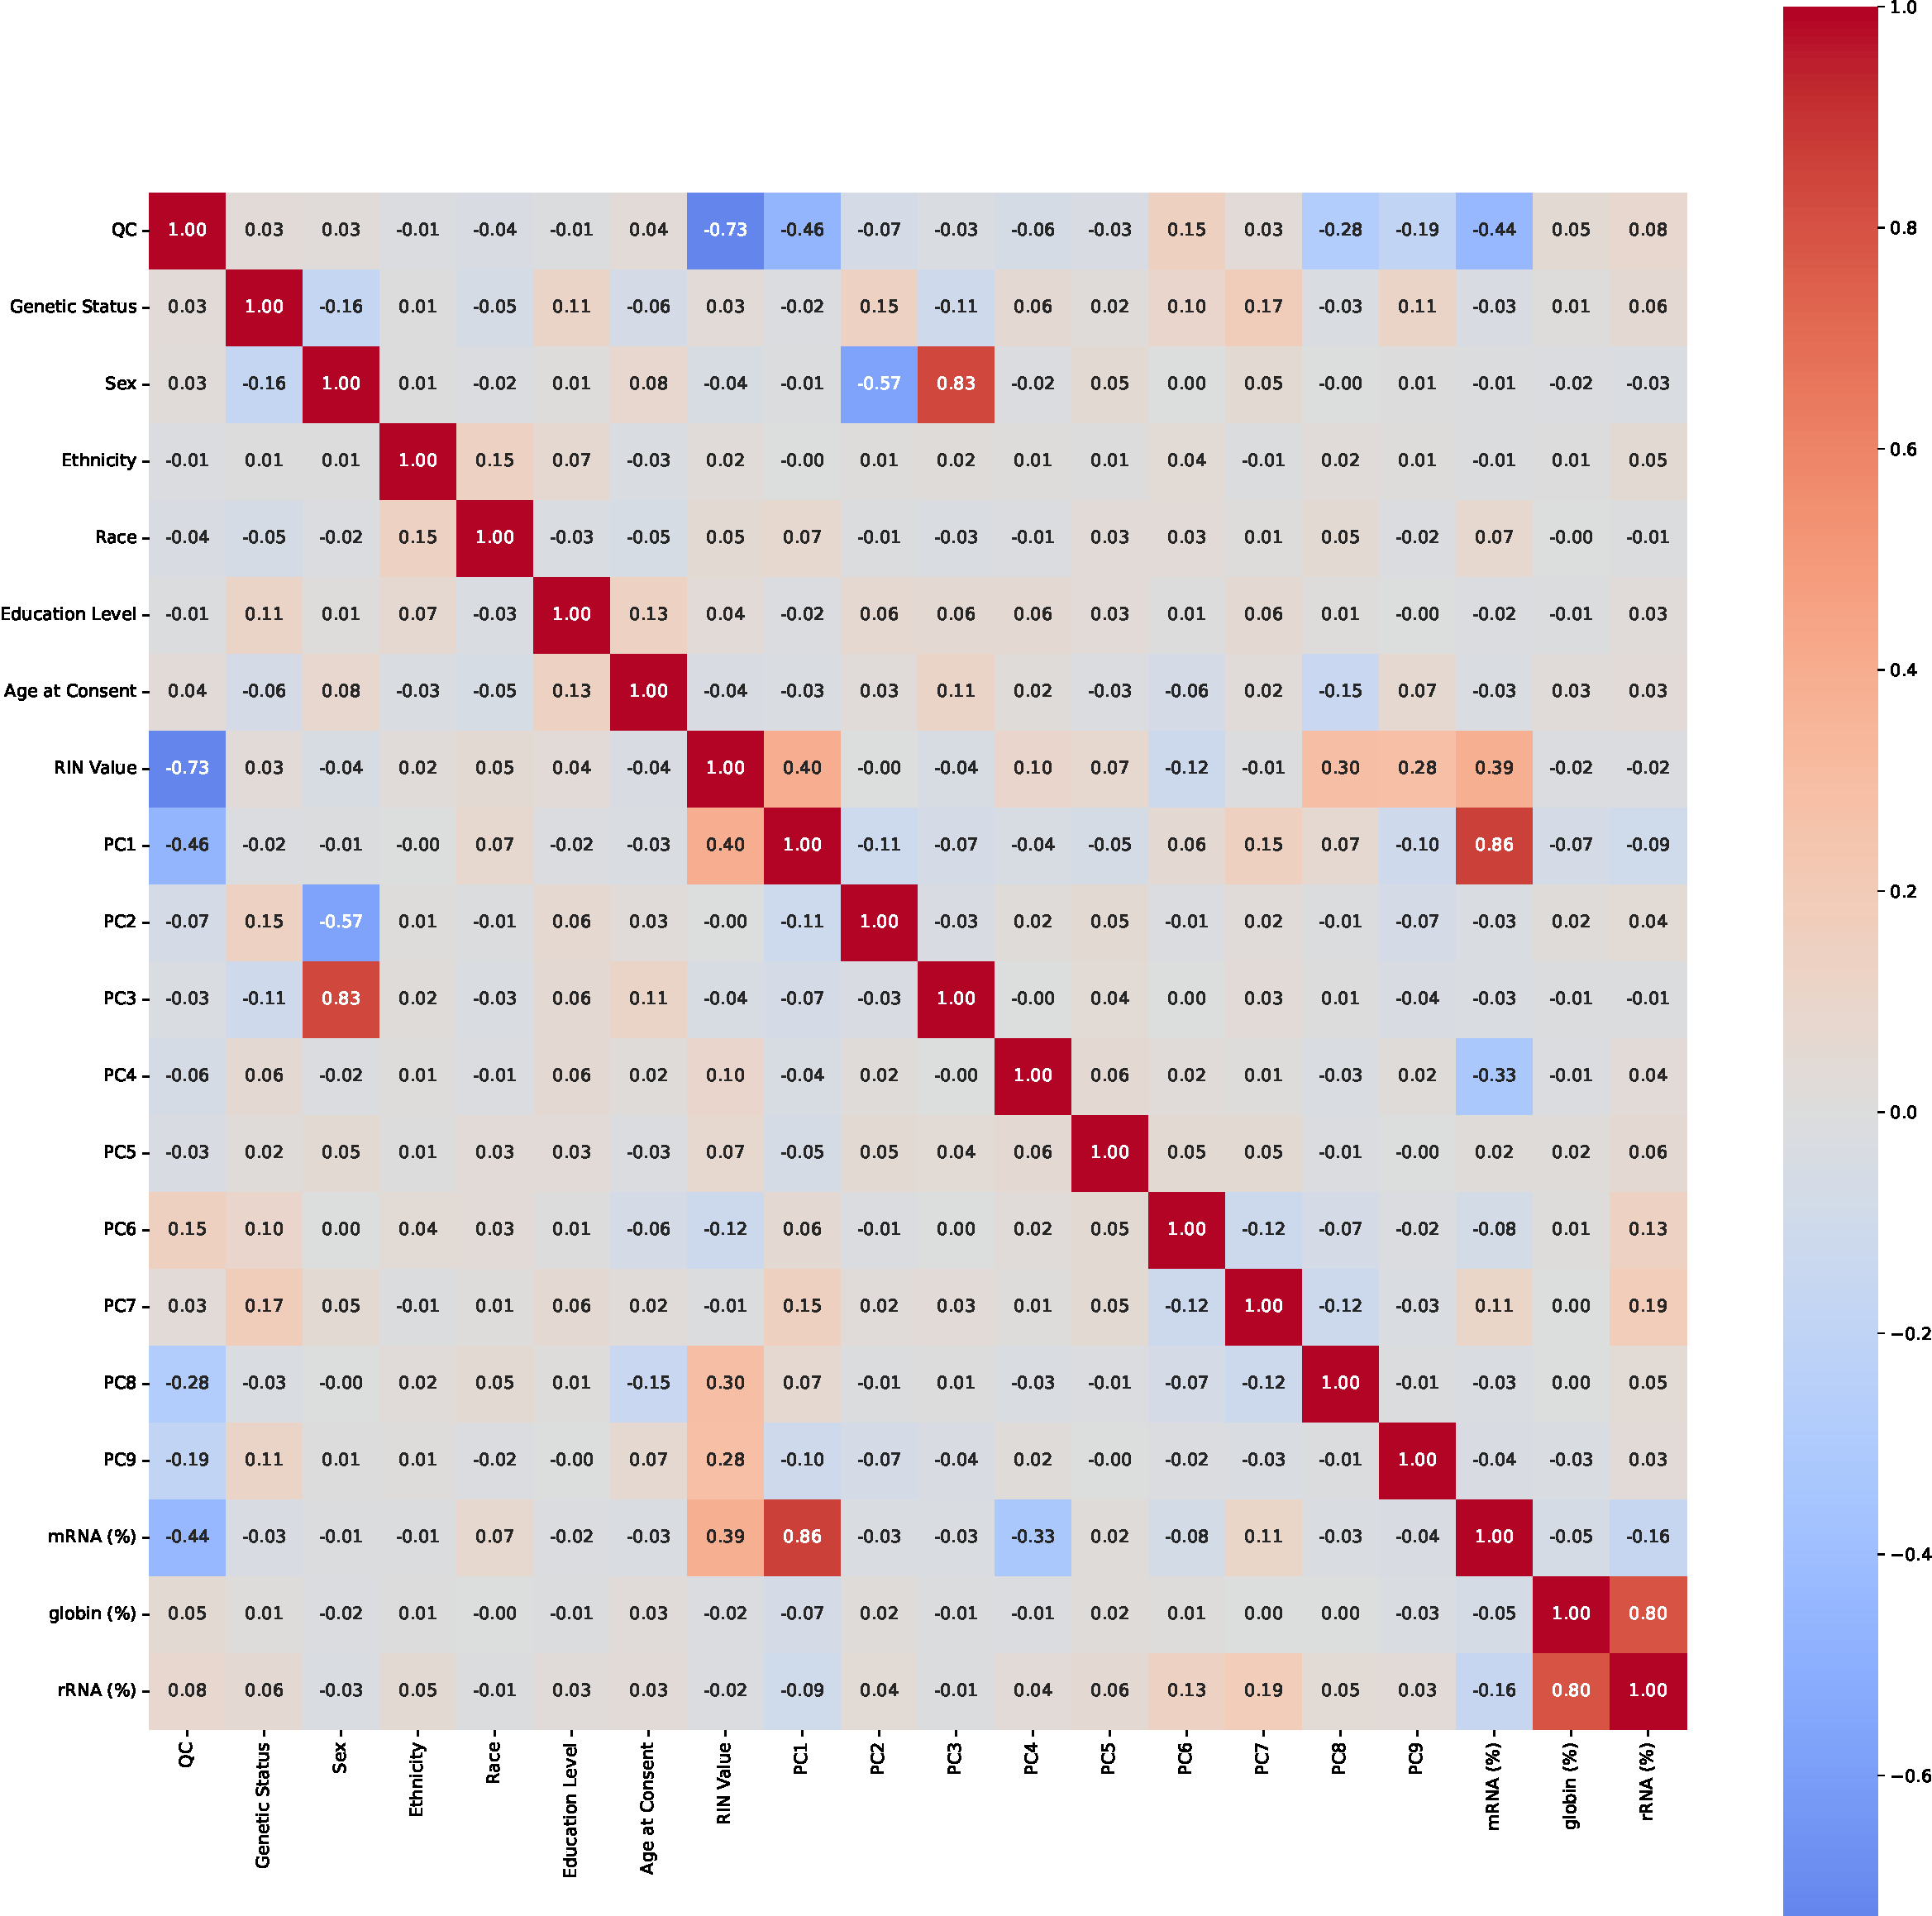
\includegraphics[width=15cm]{../../python_code/plots/filtered_correlations_meta_data.11192021.pdf}
    \end{figure}

    Visit 
    \url{https://www.ppmi-info.org/access-data-specimens/data}
    for more details on PPMI.
    %
    Note that download of the metadata CSV requires applying for the data access.


\newpage
\noindent\textbf{FNN description.}
The FNN structure was obtained by minimizing validation error rate within a small search space of hyperparameter values.
The hyperparameters considered and the associated search space boundaries are shown in \cref{tab:hparams_fnn}'s middle column.
%
\begin{table}[!h]
    \centering
    \begin{threeparttable}
    \caption{FNN hyperparameters.}
    \label{tab:hparams_fnn}
    \begin{tabular}{ccc}
        \toprule
            Hyperparameter & Possible values & Best after 100 trials \\
        \midrule
            Hidden layers' activation function & ReLU$^*$ or sigmoid & ReLU \\
            Hiddden layers' width & $\{1, 2, \dots, 16\}$ & 16 \\
            Number of hidden layers & $\{1, 2, \dots, 16\}$ & 4 \\
            Learning rate$^{**}$ & $[10^{-4}, 10^{-2}]$ & $1.88 \times 10^{-3}$\\
        \bottomrule
    \end{tabular}
    \begin{tablenotes}
        \item $^*$ Rectified Linear Unit, $f(x) = \max(0, x)$ 
        \item $^{**}$ Sampled from the log domain
    \end{tablenotes}
\end{threeparttable}
\end{table}

More precisely, the validation error corresponds to 
the number of wrong predictions made on the validation samples divided by the number of validation samples.

To find the point of minimum validation error within the hyperparameter space, the Optuna framework was used.
This tool picks a subspace of the previously defined search space, samples hyperparameters from it, and evaluates the model using those values.
The exploration of the subspace as a whole is called trial, and the model evaluations within a trial, steps.  
Trials are repeated arbitrarily, and their results are saved to guide following searches, 
with unpromising trials were stopped (pruned) early.

The FNN with smallest validation error, 4.30\%, has the parameters presented in \cref{tab:hparams_fnn}'s right column.
\Cref{fig:fnn} illustrates this network.
Trials used 15 epochs, 32 batch size, and the Adam optimizer from the Keras Python library for gradient descent calculation.
No dropout or batch normalization was applied due to the relatively small size of the neural network.

\begin{figure}[hb]
    \centering
    \caption{FNN with smallest validation error after 100 trials.}
    \label{fig:fnn}
    
\includegraphics[width=.625\linewidth]{fnn.png}
\end{figure}


\noindent\textbf{DT description.}
The DT's structure was obtained in the same fashion as the FNN's, that is,
by minimizing validation error on a hyperparameter space.
%
The hyperparameters considered and the associated search space boundaries are shown in \cref{tab:hparams_dt}.
%
The best DT with smallest validation error, 4.97\%, has the parameters presented in \cref{tab:hparams_dt}.
\Cref{fig:dt} illustrates this network.
%
\begin{table}[!h]
    \centering
    \caption{DT hyperparameters.}
    \label{tab:hparams_dt}
    \begin{tabular}{ccc}
        \toprule
            Hyperparameter & Possible values & Best after 100 trials \\
        \midrule
            Criterion & Entropy, Gini, or Log-loss & Entropy \\
            Maximum depth & $\{2, 3, \dots, 20\}$ & 4\\
        \bottomrule
    \end{tabular}
\end{table}
.
\newpage
\begin{figure}[hb]
    \centering
    \caption{DT with smallest validation error after 100 trials.}
    \label{fig:dt}
    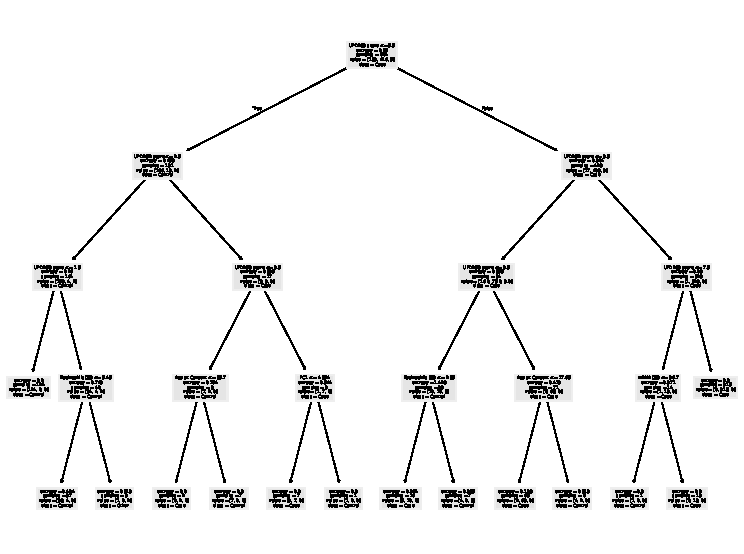
\includegraphics[width=.9\textheight, angle=90]{../../python_code/plots/dt/best_model.pdf}
\end{figure}

\clearpage
\noindent\textbf{Performance comparison.}

For a discussion on Optuna's optimization and its resulting hyperparameters, check the section at the end of this report.

\begin{figure}[!ht]
    \centering
    \caption{Confusion matrices of best FNN and DT architectures.}
    \label{fig:confusion_matrices_fnn_dt}
    \begin{subfigure}{.49\textwidth}
        \centering
        
\includegraphics[width=.8\linewidth]{../../python_code/plots/fnn/confusion_matrix.pdf}
    \end{subfigure}
    %
    \begin{subfigure}{.49\textwidth}
        \centering
        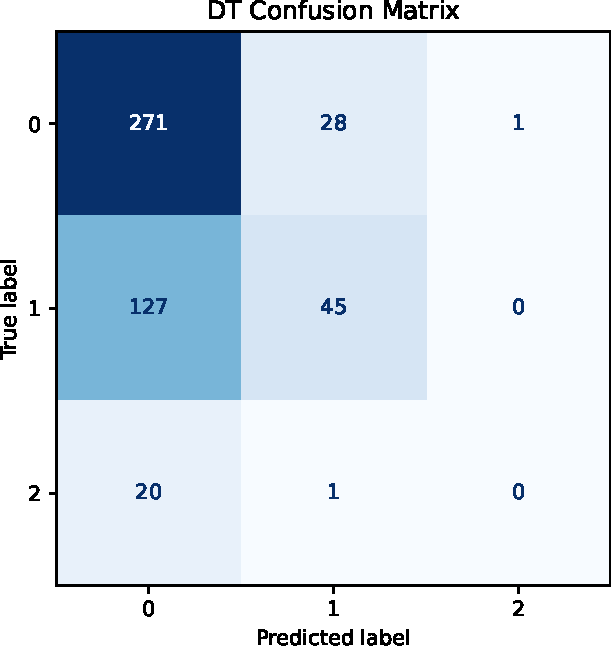
\includegraphics[width=.8\linewidth]{../../python_code/plots/dt/confusion_matrix.pdf}
    \end{subfigure}
\end{figure}